\documentclass[12pt, a4paper]{article}
\usepackage[utf8]{inputenc}
\usepackage[IL2]{fontenc}
\usepackage[czech]{babel}

\usepackage[pdftex]{hyperref}
\hypersetup{colorlinks=true,
  unicode=true,
  linkcolor=black,
  citecolor=black,
  urlcolor=black,
  bookmarksopen=true}
\usepackage{graphicx}
\usepackage{caption}
\usepackage{subcaption}
\usepackage{url}
\usepackage{placeins}

%Nastavi hloubku obsahu \setcounter{tocdepth}{3}

\begin{document}
	\begin{titlepage}
		\begin{center}
			
\includegraphics{img/ZCULogo.pdf}\\[1cm]
			\textsc{\LARGE Západočeská univerzita v~Plzni}\\[0.1cm]
			\textsc{\Large Fakulta aplikovaných věd}\\[0.1cm]
			\textsc{\large Katedra informatiky a~výpočetní techniky}
			\vfill
			\textsc{\LARGE Semestrální práce KIV/MKZ}\\[0.2cm]
			\LARGE{Studentův pomocník}
			\vfill
			Jaroslav Klaus\\[0.2cm]
			\today, Plzeň
		\end{center}
	\end{titlepage}

	\tableofcontents
	\newpage

	\section{Zadání}
	V rámci samostatné práce je potřeba vytvořit předem odsouhlasenou aplikaci na zvolené cílové platformě, předvést funkčnost aplikace v emulátoru nebo na fyzickém zařízení a odevzdat okomentovaný kód práce včetně dokumentace.
	
	Pro splnění těchto podmínek jsem si zvolil tvorbu aplikace pro platformu Android, která by měla sloužit jako pomocník pro studenta vysoké školy, na které je používán informační systém \emph{IS/STAG}. Aplikace bude zobrazovat rozvrh studenta získaný z~\emph{IS/STAGu} po dnech a dovolí mu si ke každému z~předmětů zobrazit či přidat další informace, jako jsou
		\begin{itemize}
			\item sylabus předmětu,
			\item podmínky pro splnění předmětu,
			\item úkoly, které je potřeba udělat
			\item a~počet absencí v~předmětu.
		\end{itemize}
	
	\section{Programátorská dokumentace}
		\subsection{Uložení dat}
		Data jako rozvrhy a~sylaby předmětů jsou uloženy v~XML souborech ve složkách strukturou vycházející z~webové adresy, ze které byly získány, a~osobního čísla rozvrhu. Pro jejich čtení a~parsování byla vytvořena třída \texttt{ParseXmls}, která využívá třídu \texttt{XmlPullParser}.
		
		Konfigurační položky a~záznamy o~tom, jaké rozvrhy jsou dostupné, jsou uloženy ve~sdílených preferenčních souborech. To jsou typicky také XML soubory, ale o~jejich čtení a~ukládání se stará poskytované Android API.
		
		Data o~podmínkách a~úkolech se uchovávají v~databázi v~příslušných tabulkách. K~manipulaci s~nimi jsou vytvořené třídy \texttt{TasksDatabaseHelper} a~\texttt{TermsDatabaseHelper} odděděné od \texttt{SQLiteOpenHelper}.
		
		Veškerá práce s~daty a~jiné eventuálně časově náročné akce jsou prováděny v~jiných vláknech pomocí třídy \texttt{AsyncTask}.
		
		\subsection{Hlavní obrazovka}
		Hlavní obrazovka \texttt{MainActivity} zobrazuje předměty po jednotlivých dnech, proto byla implementována pomocí \texttt{Tabbed Activity} s~volbou \texttt{Action Bar Tabs (with ViewPager)}. Základem jsou tedy \uv{záložky} se dny zobrazující fragmenty, o~jejichž změnu se stará třída \texttt{ViewPager} a~její adaptér odděděný od třídy \texttt{FragmentStatePagerAdapter}.
		
		Tento adaptér vytváří fragment \texttt{DayFragment}, který v~prvku \texttt{Expandable-\\ListView} zobrazuje rozvrh pro daný den. Pro to je však potřeba další adaptér (\texttt{BaseExpandableListAdapter}), který je použit pro zobrazení údajů o~předmětu v~prvku \texttt{ExpandableListView}.
		
		Při vytvoření aplikace se z~konfiguračních souborů zjistí poslední nastavení a~podle toho se načte příslušný rozvrh do struktur. Poté se naplní prvek \texttt{Spinner} dostupnými staženými rozvrhy. Tento prvek slouží ke změně zobrazovaného rozvrhu.
		
		\subsection{Přidání rozvrhu}
		Aktivita pro přidání rozvrhu \texttt{AddTimetableActivity} je základní aktivita vytvořená jako \texttt{Basic Activity}. Obsahuje tři prvky: \texttt{Spinner}, \texttt{EditText} a~\texttt{Button}.
		
		\texttt{Spinner} slouží pro výběr školy a~je pro něj vytvořen adaptér pomocí \texttt{ArrayAdapter\textless String\textgreater}, který umožňuje nejen zobrazení názvu školy, ale i~jejího loga.
		
		\texttt{EditText} je vstupní pole sloužící pro zadání osobního čísla studenta, jehož rozvrh má být přidán.
		
		\texttt{Button} je tlačítko, které slouží pro zahájení akce přidání nového rozvrhu.
		
		Pro stahování souborů se využívá tříd \texttt{URL}, \texttt{URLConnection}, \texttt{Buffered-\\InputStream} a~\texttt{FileOutputStream}.
		
		\subsection{Odebrání rozvrhu}
		Pro odebrání rozvrhů se využívá třídy \texttt{AlertDialog.Builder}, pomocí které se vytvoří dialog se zatrhávacími políčky u~osobních čísel (metodou \texttt{setMulti-\\ChoiceItems()}). Vybrané položky se poté vymažou.
		
		\subsection{Nastavení}
		Aktivita nastavení \texttt{SettingsActivity} obsahuje pouze dvě položky, a~to pro změnu osobního čísla a~semestru. Obě položky jsou realizovány pomocí prvku \texttt{ListPreference}.
		
		\subsection{Zobrazení sylabu}
		Aktivita pro zobrazení sylabu předmětu je vytvořena jako \texttt{Basic Activity}. Obsahuje pouze prvky \texttt{TextView}, které slouží pro zobrazení příslušných informací o~předmětu.
		
		\subsection{Podmínky a úkoly}
		Aktivita pro zobrazení podmínek \texttt{TasksActivity} a úkolů \texttt{TermsActivity} je upravená \texttt{Basic Activity}, která v~prvku \texttt{ListView} zobrazuje podmínky načtené z~databáze. Využívá k~tomu adaptér typu \texttt{ArrayAdapter\textless Term\textgreater} a \texttt{ArrayAdapter\textless Task\textgreater}, který slouží k~vytvoření a~nastavení hodnot zobrazovaných prvků.
		
		Pro vytvoření nového prvku je použito tlačítko \texttt{FloatingActionButton}, které spustí aktivitu \texttt{AddTermActivity} nebo \texttt{AddTaskActivity}. Stejná aktivita se spustí pro úpravu existující podmínky nebo úkolu a~to tak, že se na danou podmínku či úkol klikne.
		
		Pro smazání podmínky nebo úkolu stačí dlouze zmáčknout na danou podmínku či úkol a~potvrdit dialog pro smazání. Dialog je vytvořen pomocí třídy \texttt{AlertDialog.Builder}.
		
		\subsection{Absence}
		Aktivita pro zobrazení a~úpravu absencí je opět \texttt{Basic Activity}. Obsahuje dva prvky -- \texttt{NumberPicker} pro zobrazení a~výběr počtu absencí v~předmětu a~tlačítko, které slouží pro nastavení nově vybrané hodnoty.
	
	\section{Uživatelská dokumentace}
		\subsection{Hlavní obrazovka}
		První aktivní prvek na hlavní obrazovce (pokud jdeme zleva doprava, shora dolu) slouží pro výběr zobrazovaného rozvrhu. Pokud máme více stažených rozvrhů, zobrazí se po kliknutí na tento prvek, viz obrázek \ref{personalNumbers}.
		
		Další v~pořadí je tlačítko pro přidání nového rozvrhu. Má tvar \uv{plus} a~případně může být skryto v~nabídce menu (obrázek \ref{menu}) s~názvem \emph{Přidat rozvrh}. Stejně tak další tlačítko, které má tvar \uv{minus}, může mít název \emph{Vymazat rozvrhy} a slouží ke smazání rozvrhů.
		
		V~nabídce menu se poté ukrývá tlačítko pro otevření nastavení aplikace a~další pro zobrazení informací o~aplikaci.
		
		Na hlavní obrazovce se zobrazuje rozvrh studenta po jednotlivých dnech, viz obrázek \ref{main}. Pro změnu zobrazovaného dnu slouží pás záložek s~názvy dnů, přičemž stačí na požadovaný den kliknout. Další možností je přejet na den vedle (provést tzv. \uv{swipe} zleva doprava, případně zprava doleva).
		
		\begin{figure}[ht!]
			\centering
			\caption{Hlavní obrazovka}
			\label{main}
			\begin{subfigure}{.5\textwidth}
				\centering
				\caption{Bez rozvrhu}
				\label{mainWithout}
				
\includegraphics[width=6.5cm]{img/mainWithoutTimetable.png}
			\end{subfigure}%
			\begin{subfigure}{.5\textwidth}
				\centering
				\caption{S~rozvrhem}
				\label{mainWith}
				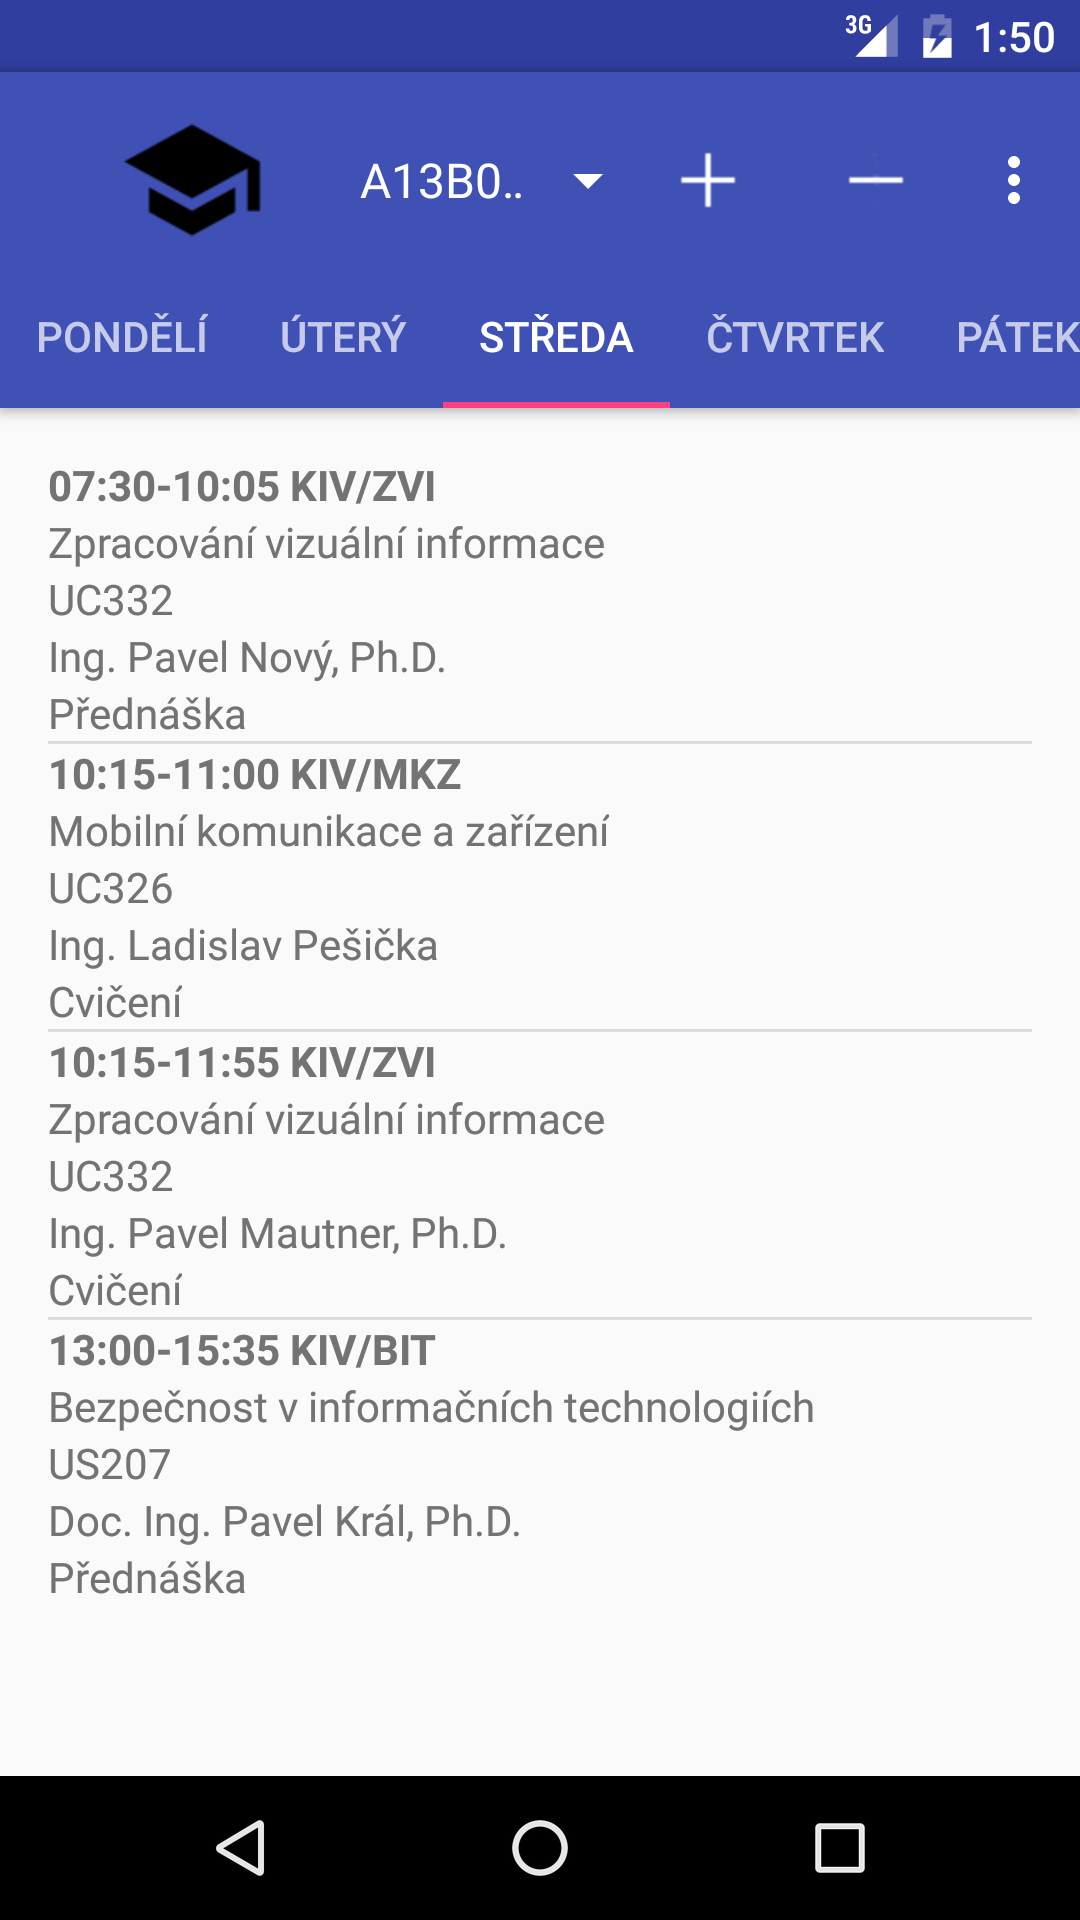
\includegraphics[width=6.5cm]{img/mainWithTimetable.png}
			\end{subfigure}
			\begin{subfigure}{.5\textwidth}
				\centering
				\caption{Výběr rozvrhu}
				\label{personalNumbers}
				
\includegraphics[width=6.5cm]{img/personalNumbers.png}
			\end{subfigure}%
			\begin{subfigure}{.5\textwidth}
				\centering
				\caption{Menu aplikace}
				\label{menu}
				
\includegraphics[width=6.5cm]{img/menu.png}
			\end{subfigure}
		\end{figure}
		
		Pro zpřístupnění akcí u~předmětu stačí na daný předmět kliknout a~zobrazí se dostupné akce jako na obrázku \ref{subjectActions}. Akce se vždy vztahují pouze k~danému předmětu, takže například po kliknutí na \emph{Úkoly} u~předmětu \emph{KIV/MKZ} se zobrazí pouze úkoly z~předmětu \emph{KIV/MKZ}.
		
		\begin{figure}[ht!]
			\centering
			\caption{Dostupné akce po kliknutí na předmět}
			\label{subjectActions}
			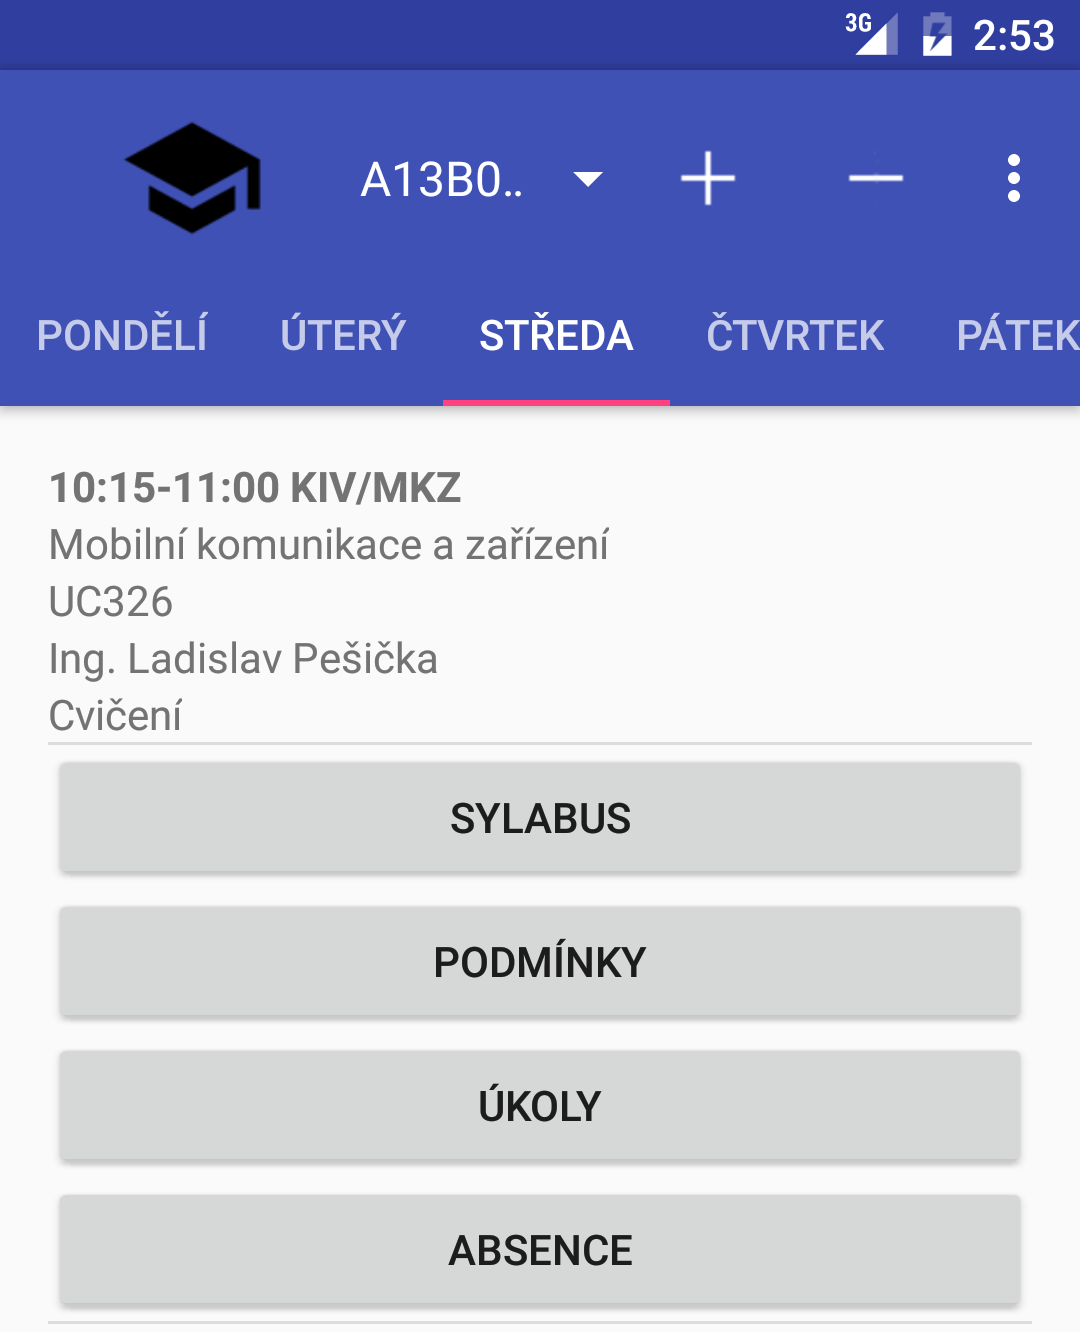
\includegraphics[width=6.5cm]{img/subjectActions.png}
		\end{figure}
		\FloatBarrier
		
		\subsection{Přidání rozvrhu}
		Pro přidání rozvrhu slouží tlačítko \uv{plus} na hlavní obrazovce, které také může být skryté v~nabídce menu a~pojmenované \emph{Přidat rozvrh}. Po jeho stisknutí se otevře aktivita, ve které musíme vybrat školu a~zadat osobní číslo studenta, jehož rozvrh chceme přidat. Po zadání a~stisknutí tlačítka \emph{Přidat} se stáhnou z~\emph{IS/STAGu} dané školy potřebné soubory a~rozvrh se zobrazí, tak jako na obrázku \ref{mainWith}.
		
		\begin{figure}[ht!]
			\centering
			\caption{Aktivita pro přidání rozvrhu}
			\label{addTimetable}
			
\includegraphics[width=6.5cm]{img/addTimetable.png}
		\end{figure}
		\FloatBarrier
		
		\subsection{Odstranění rozvrhů}
		Pokud chceme některé rozvrhy odstranit, stiskneme tlačítko \uv{minus} na hlavní obrazovce. Otevře se dialog se všemi dostupnými rozvrhy, ve kterém vybereme ty, které chceme odstranit, viz obrázek \ref{deleteTimetables}. Potvrdíme stisknutím tlačítka \emph{OK} a~vybrané rozvrhy a~jejich soubory budou odstraněny.
		
		\begin{figure}[ht!]
			\centering
			\caption{Dialog pro odstranění rozvrhů}
			\label{deleteTimetables}
			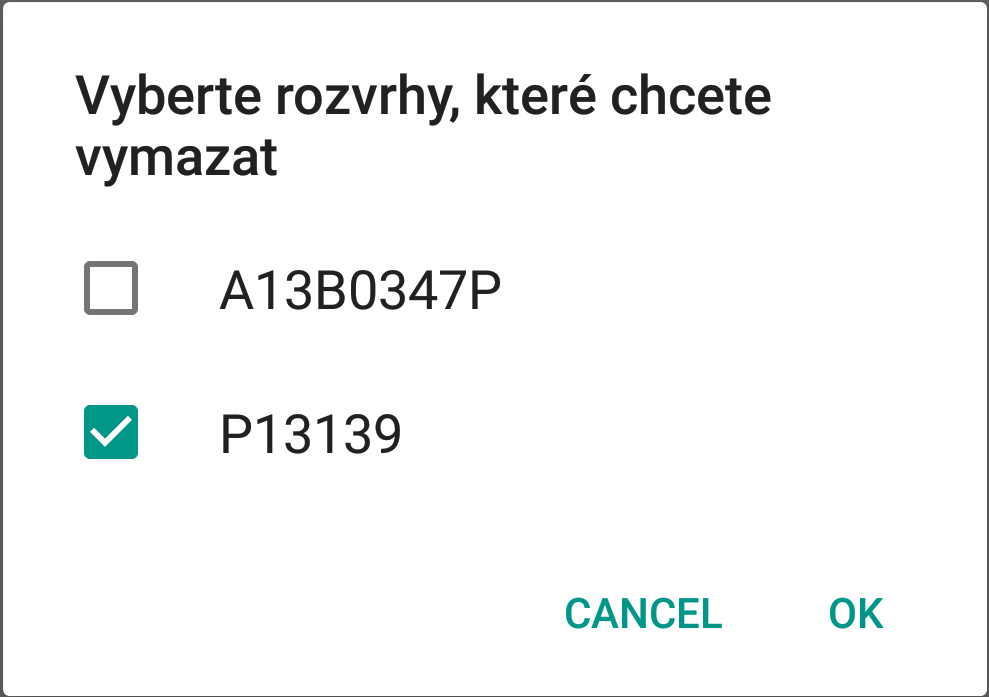
\includegraphics[width=6.5cm]{img/deleteTimetables.png}
		\end{figure}
		\FloatBarrier
		
		\subsection{Nastavení}
		Pro přístup do nastavení aplikace zvolíme v~menu položku \emph{Nastavení}. Ta obsahuje dva prvky, které je možné nastavit, viz obrázek \ref{settings}. Prvním je osobní číslo, jehož rozvrh chceme zobrazit. Druhým je semestr, pro který chceme rozvrh zobrazit. 
		
		\begin{figure}[ht!]
			\centering
			\caption{Nastavení aplikace}
			\label{settings}
			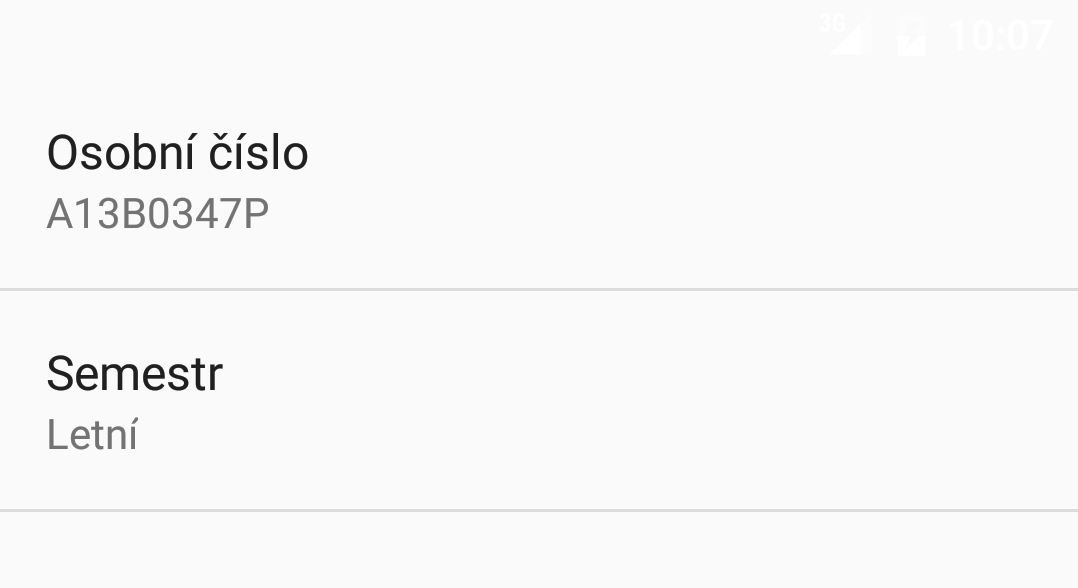
\includegraphics[width=6.5cm]{img/settings.png}
		\end{figure}
		\FloatBarrier
		
		\subsection{O aplikaci}
		Poslední položkou menu je položka \emph{O aplikaci}. Ta zobrazí aktivitu s~logem \emph{IS/STAG} a~informacemi o~aplikaci, viz obrázek \ref{about}.
		
		\begin{figure}[ht!]
			\centering
			\caption{O aplikaci}
			\label{about}
			
\includegraphics[width=6.5cm]{img/about.png}
		\end{figure}
		\FloatBarrier
		
		\subsection{Sylabus}
		Po kliknutí na akci \emph{Sylabus} se zobrazí sylabus předmětu, viz obrázek \ref{syllabus}. V~této aktivitě nejsou žádné aktivní prvky a~slouží pouze k~poskytnutí informací o~předmětu.
		
		\begin{figure}[ht!]
			\centering
			\caption{Sylabus předmětu KIV/MKZ}
			\label{syllabus}
			
\includegraphics[width=6.5cm]{img/syllabus.png}
		\end{figure}
		\FloatBarrier
		
		\subsection{Podmínky}
		Kliknutím na akci \emph{Podmínky} u~předmětu zobrazíme aktivitu s~výčtem již přidaných podmínek daného předmětu, viz obrázek \ref{termsList}. Zde se zobrazuje jak název podmínky, tak její popis, přičemž název musí být vždy zadán.
		
			\subsubsection{Přidání podmínky}
			Pro přidání podmínky slouží tlačítko \uv{plus} v~pravém dolním rohu obrazovky. Po kliknutí na něj se zobrazí aktivita pro přidání nové podmínky, viz \ref{addTerm}. Povinný je název podmínky, popis může zůstat prázdný. Pokud tedy zadáme název, případně popis a~stiskneme tlačítko \emph{Přidat podmínku}, podmínka se vloží do databáze a~zobrazí se v~seznamu podmínek.
			
			\subsubsection{Upravení podmínky}
			Pro upravení podmínky musíme danou podmínku najít v~seznamu podmínek a~kliknout na ni. Otevře se stejná aktivita jako pro přidání nové podmínky s~tím rozdílem, že budou předvyplněny položky tak, jak byly uloženy pro danou podmínku. Po provedení požadovaných úprav stačí kliknout na tlačítko \emph{Přidat podmínku}, což provede aktualizaci záznamu v~databázi a~v~seznamu podmínek se již bude zobrazovat upravená podmínka.
			
			\subsubsection{Smazání podmínky}
			Pro smazání podmínky je potřeba danou podmínku najít a~dlouze na ní kliknout. Poté se zobrazí dialog \ref{deleteTerm}, který je pro smazání potřeba potvrdit kliknutím na tlačítko \emph{Ano}.
		
			\begin{figure}[ht!]
				\centering
				\caption{Podmínky předmětu KIV/MKZ}
				\label{terms}
				\begin{subfigure}{.5\textwidth}
					\centering
					\caption{Seznam podmínek}
					\label{termsList}
					
\includegraphics[width=6.5cm]{img/terms.png}
				\end{subfigure}%
				\begin{subfigure}{.5\textwidth}
					\centering
					\caption{Vytvoření nové podmínky}
					\label{addTerm}
					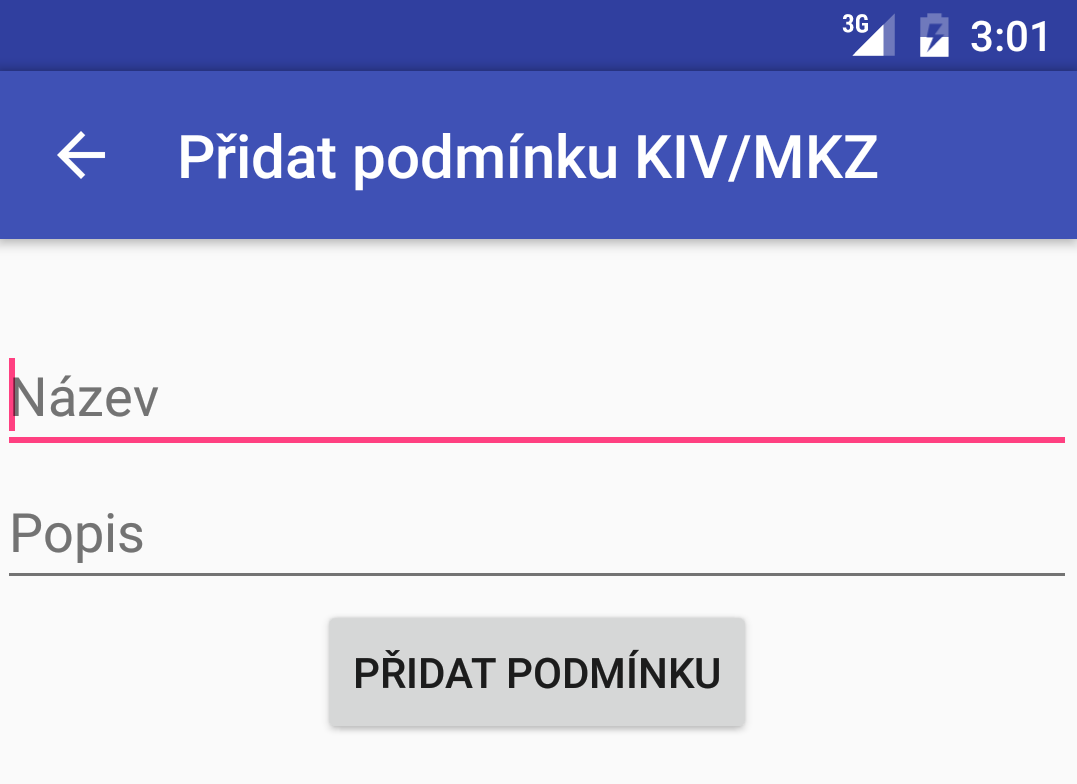
\includegraphics[width=6.5cm]{img/addTerm.png}
				\end{subfigure}
				\begin{subfigure}{.5\textwidth}
					\centering
					\caption{Dialog pro potvrzení smazání podmínky}
					\label{deleteTerm}
					
\includegraphics[width=6.5cm]{img/deleteTerm.png}
				\end{subfigure}
			\end{figure}
			\FloatBarrier
		
		\subsection{Úkoly}
		Po kliknutí na akci \emph{Úkoly} u~předmětu zobrazíme aktivitu s~výčtem již přidaných úkolů daného předmětu, viz obrázek \ref{tasksList}. Zde se zobrazuje jak název úkolu, jeho popis, tak datum a~čas, do kdy se má úkol splnit, přičemž název musí být vždy zadán.
		
			\subsubsection{Přidání úkolu}
			Pro přidání úkolu slouží tlačítko \uv{plus} v~pravém dolním rohu obrazovky. Po kliknutí na něj se zobrazí aktivita pro přidání nového úkolu, viz \ref{addTask}. Povinný je název úkolu. Popis může zůstat prázdný a~datum a~čas se automaticky vyplní na aktuální hodnotu. Pro změnu data a~času se po kliknutí na dané pole otevře dialog pro výběr, viz \ref{dateDiaog} a~\ref{timeDialog}. Pokud tedy zadáme název, případně popis, datum a~čas a~stiskneme tlačítko \emph{Přidat úkol}, úkol se vloží do databáze a~zobrazí se v~seznamu.
			
			\subsubsection{Upravení úkolu}
			Pro upravení úkolu musíme daný úkol najít v~seznamu a~kliknout na něj. Otevře se stejná aktivita jako pro přidání nového úkolu s~tím rozdílem, že budou předvyplněny položky tak, jak byly uloženy pro daný úkol. Po provedení požadovaných úprav stačí kliknout na tlačítko \emph{Přidat úkol}, což provede aktualizaci záznamu v~databázi a~v~seznamu úkolů se již bude zobrazovat upravený úkol.
			
			\subsubsection{Smazání úkolu}
			Pro smazání úkolu je potřeba daný úkol najít a~dlouze na něj kliknout. Poté se zobrazí dialog \ref{deleteTask}, který je pro smazání potřeba potvrdit kliknutím na tlačítko \emph{Ano}.
		
			\begin{figure}[ht!]
				\centering
				\caption{Úkoly k~předmětu KIV/MKZ}
				\label{tasks}
				\begin{subfigure}{.5\textwidth}
					\centering
					\caption{Seznam úkolů}
					\label{tasksList}
					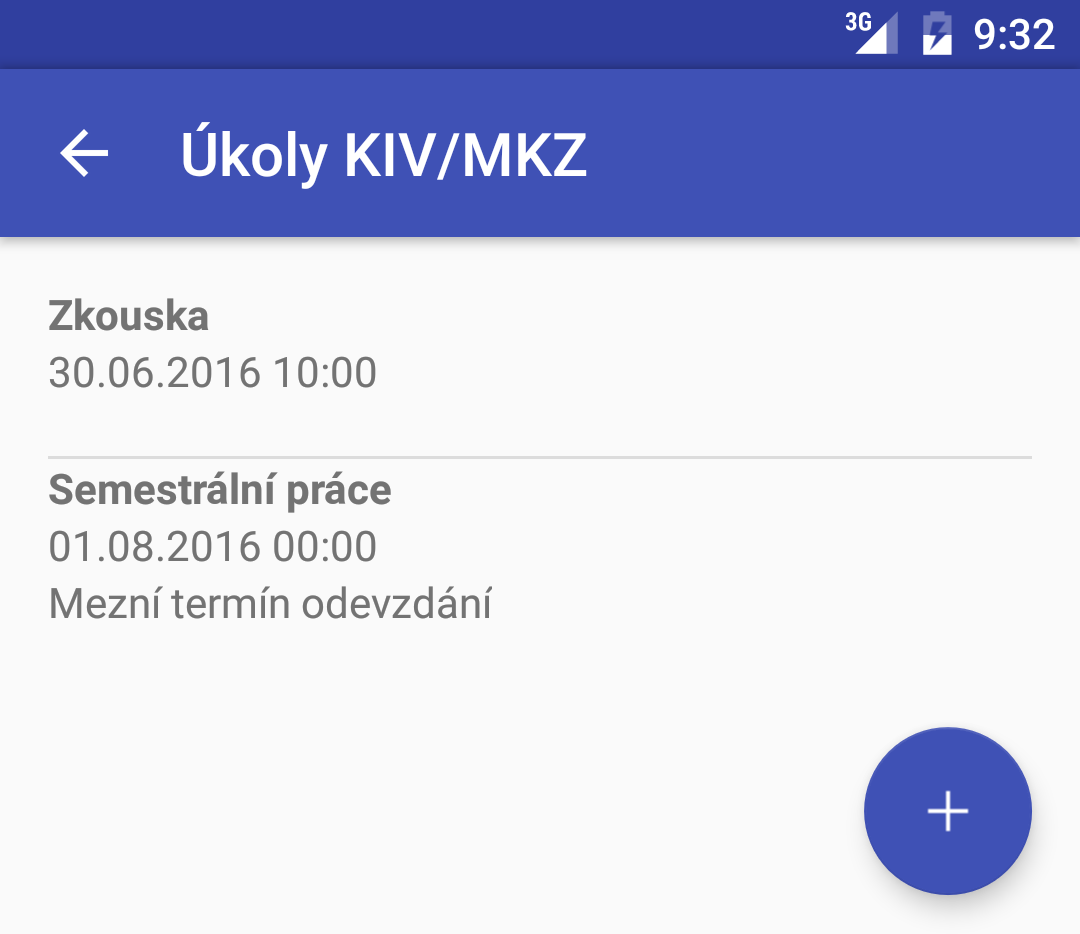
\includegraphics[width=6.5cm]{img/tasks.png}
				\end{subfigure}%
				\begin{subfigure}{.5\textwidth}
					\centering
					\caption{Vytvoření nového úkolu}
					\label{addTask}
					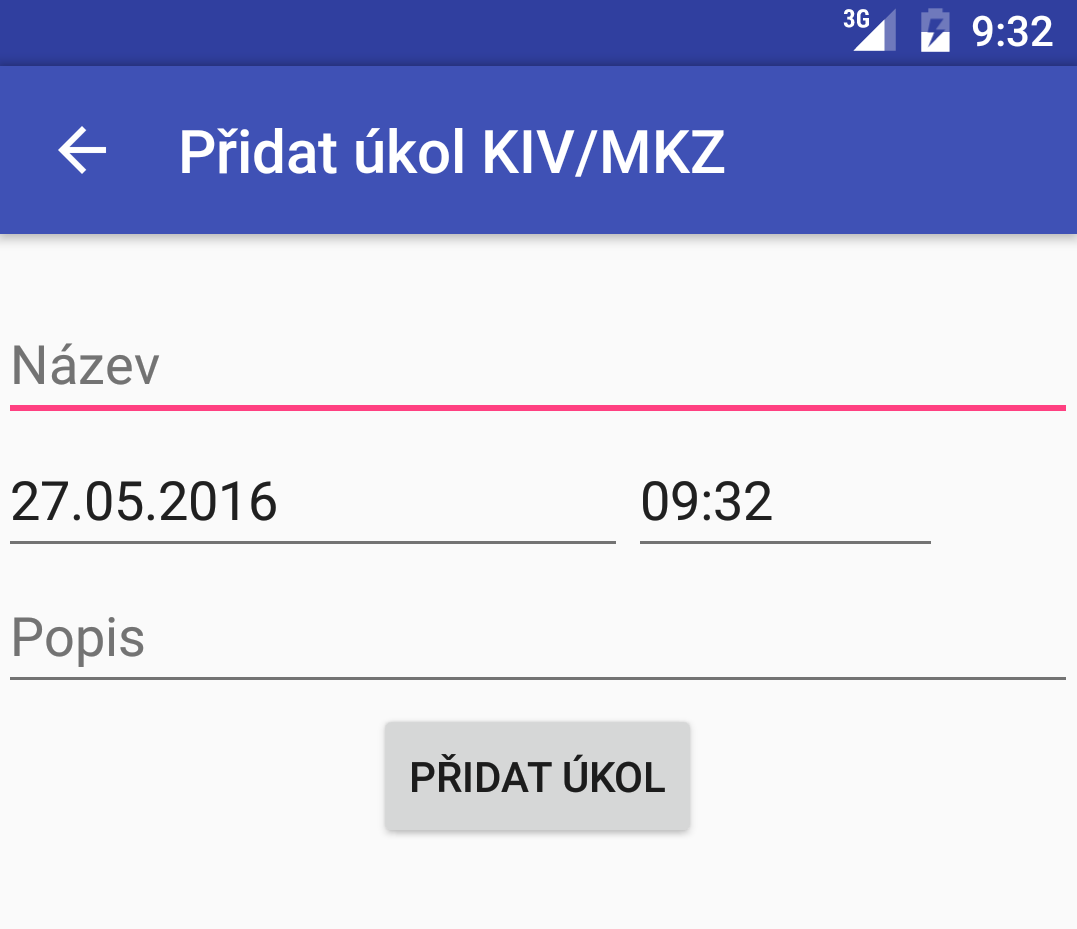
\includegraphics[width=6.5cm]{img/addTask.png}
				\end{subfigure}
				\begin{subfigure}{.5\textwidth}
					\centering
					\caption{Dialog pro výběr data úkolu}
					\label{dateDiaog}
					
\includegraphics[width=6.5cm]{img/dateDialog.png}
				\end{subfigure}%
				\begin{subfigure}{.5\textwidth}
					\centering
					\caption{Dialog pro výběr času úkolu}
					\label{timeDialog}
					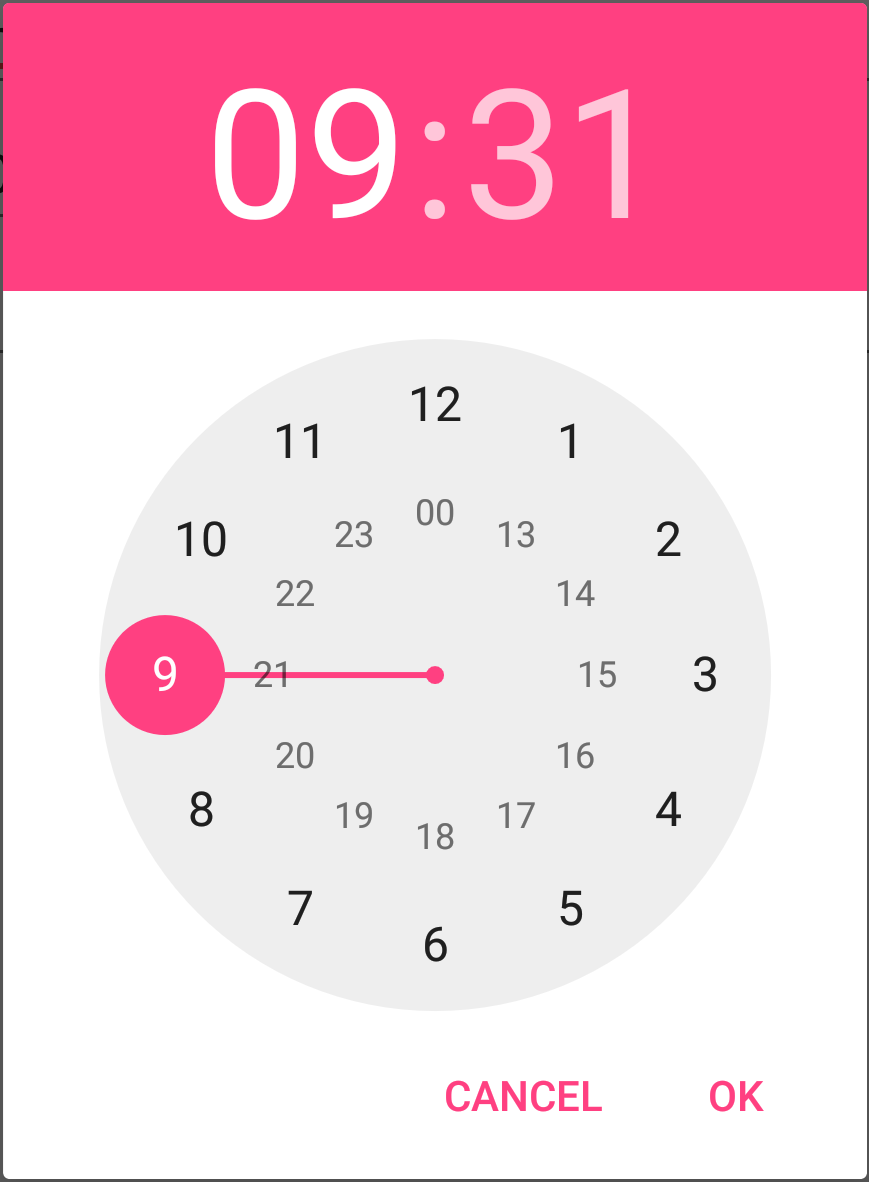
\includegraphics[width=6.5cm]{img/timeDialog.png}
				\end{subfigure}
				\begin{subfigure}{.5\textwidth}
					\centering
					\caption{Dialog pro potvrzení smazání úkolu}
					\label{deleteTask}
					
\includegraphics[width=6.5cm]{img/deleteTask.png}
				\end{subfigure}
			\end{figure}
			\FloatBarrier
			
		\subsection{Absence}
		Po kliknutí na \emph{Absence} u~předmětu zobrazíme aktivitu, v~níž se zároveň zobrazuje již uložený počet absencí a~zároveň slouží pro jeho změnu, viz \ref{absences}. Pokud tedy chceme provést změnu počtu absencí, vybereme tahem požadované číslo a~stiskneme tlačítko \emph{Upravit absence}. Tím se uloží aktuálně vybraná hodnota na číselníku.
		
		\begin{figure}[ht!]
			\centering
			\caption{Absence předmětu KIV/MKZ}
			\label{absences}
			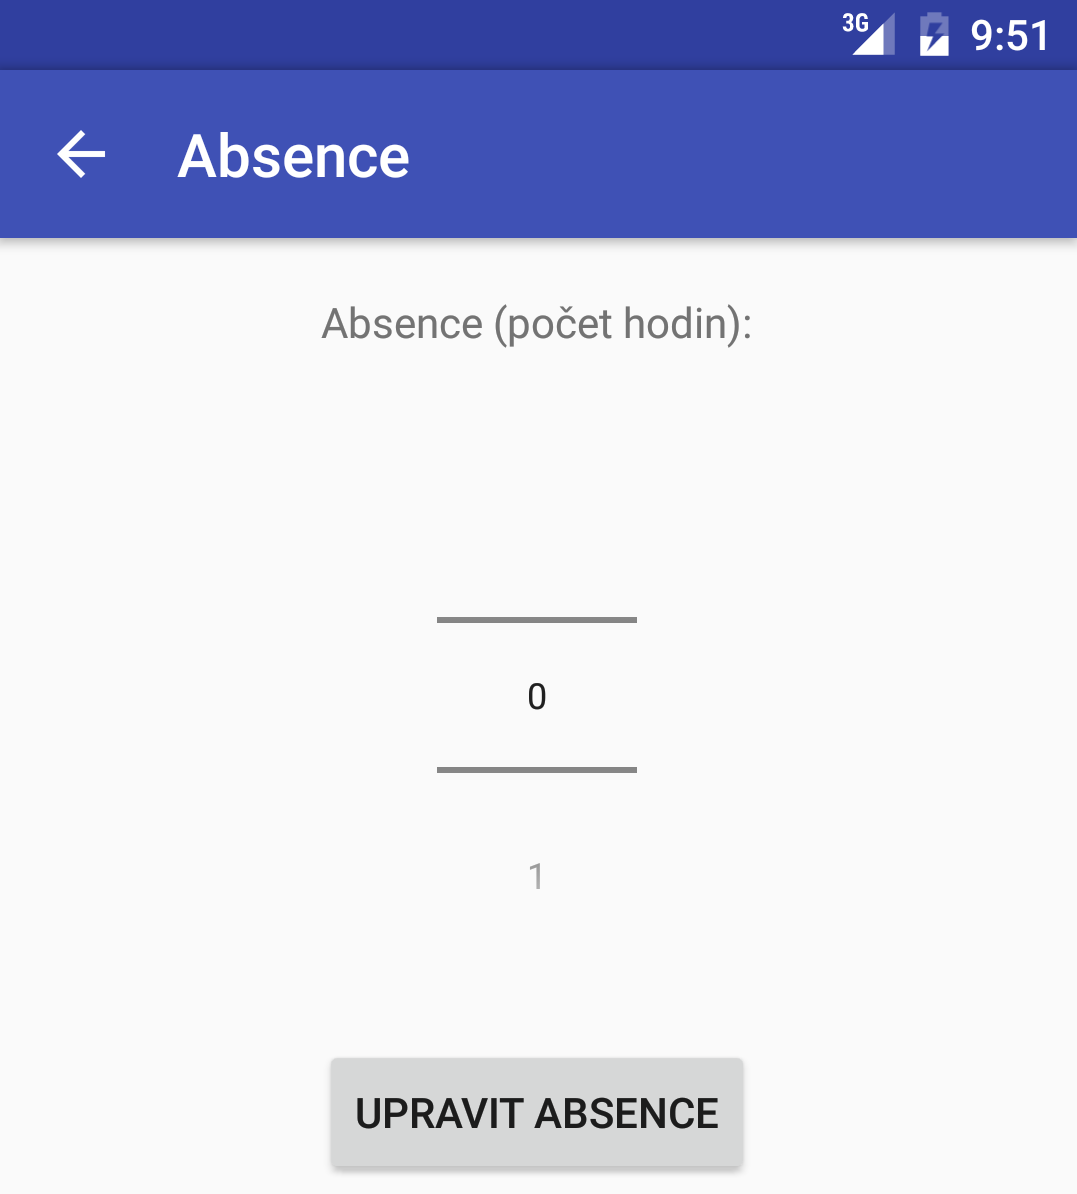
\includegraphics[width=6.5cm]{img/absences.png}
		\end{figure}
		\FloatBarrier
	
	\section{Řešené problémy}
	Během vytváření aplikace jsem narazil na několik problémů. Většina z~nich byla způsobena velmi komplikovaným životním cyklem Android aplikace, ale některé také neočekávaným chováním některých komponent.
	
		\subsection{ExpandableListView}
		Jedním z~problémů bylo, že po změně rozvrhu se neaktualizoval prvek \texttt{Expan-\\dableListView} tak, jak jsem očekával. Během tvorby a~zkoušení různých návodů z~internetu jsem narazil na tři fáze:
			\begin{enumerate}
				\item Ke změnám nedocházelo vůbec.
				\item Naprosto nedeterministické chování. Při každé změně se projevil jeden z~následujících stavů, ale vždy naprosto náhodně.
				\item Změna pouze aktuálního dne. Po změně se korektně zobrazily předměty aktuálně prohlíženého dne, ale předměty dnů okolních zůstaly ze starého rozvrhu (např. úterý se zobrazilo korektně, ale pondělí a~středa nikoli). Změny se projevily až po zobrazení dne, který byl \uv{ob jeden} dále.
			\end{enumerate}
		Konečným řešením pro mě bylo to, že jsem v~metodě \texttt{onResume()} fragmentu \texttt{DayFragment} vždy nastavoval \texttt{ExpandableListView} nový adaptér a~po načtení rozvrhu zavolal metodu \texttt{getAdapter().notifyDataSetChanged()} třídy \texttt{ViewPager}.
		
		\subsection{TabLayout}
		Dalším problémem je, že pokud přecházíme mezi dny tzv. \uv{swipem}, tak se může stát, že není vidět záložka s~aktuálně zobrazovaným dnem. Ačkoli je \texttt{TabLayout} obalen pomocí \texttt{HorizontalScrollView}, což umožňuje manuální posun, automatický posun jsem nenalezl. Tento problém jsem však neřešil, neboť není natolik závažný, aby bránil v~používání aplikace.
	
	\section{Testování}
	Aplikace byla testována na dvou emulátorech, dvou fyzických zařízeních a~několika dalších, ačkoli z~těchto dalších nemám dostupné podrobnější informace.
	
		\begin{itemize}
			\item \textbf{Emulátor Nexus 5, Android 6.0} -- Aplikace funguje bez potíží, žádné chyby ani pády jsem nezaznamenal.
			\item \textbf{Emulátor Nexus 7, Android 4.1} -- Aplikace funguje bez potíží, žádné chyby ani pády jsem nezaznamenal.
			\item \textbf{BlackBerry Z30, BlackBerry OS 10, Android Runtime 4.3} -- Ačkoli toto zařízení nemá OS Android, obsahuje Android Runtime ve verzi 4.3. I~na tomto zařízení aplikace funguje bez potíží, žádné chyby ani pády jsem nezaznamenal.
			\item \textbf{Samsung Galaxy Core Prime, Android 4.4} -- Aplikace funguje bez potíží, žádné chyby ani pády jsem nezaznamenal.
		\end{itemize}
	
	\section{Závěr}
	Vývoj aplikací pro Android je relativně složitý v~důsledku velmi komplikovaného životního cyklu aplikací a~nestandardního či neočekávaného chování některých komponent. Avšak i~přes tento fakt se mi podařilo vytvořit funkční a~snad i~užitečnou aplikaci, která splňuje zadání semestrální práce KIV/MKZ.
	
	Tvorba aplikace byla velmi náročná, zabrala mi přibližně 120-150 hodin práce. Největší podíl na tom měl návrh aplikace a~seznámení se s~použitými komponentami. Také řešení problémů zabralo značnou část času.
	
	Věřím, že aplikace by mohla najít využití u~studentů vysokých škol, proto bych ji chtěl zveřejnit na \emph{Google Play} a~nadále udržovat, případně i~přidávat další funkce, jako např. zapisování na zkoušky apod.
	
	\newpage
	\begin{thebibliography}{9}
		\bibitem{prednasky}
			Ing. Ladislav Pešička,
			Mobilní komunikace a zařízení,
			Přednášky,
			2016,
			\url{https://cw.zcu.cz/portal/studium/courseware/kiv/mkz/prednasky.html}
			
		\bibitem{android}
			Google Inc.,
			API Guides,
			2016,
			\url{https://developer.android.com/guide/index.html}
	\end{thebibliography}
	
\end{document}